%%%%%%%%%%%%%%%%%%%%%%%%%%%%%%%%%%%%%%
  %%%%%%%%%%%%%%%%%%%%%%%%%%%%%%%%%%%%%%
  % Do not edit the TeX file your work
% will be overwritten.  Edit the RnW
% file instead.
%%%%%%%%%%%%%%%%%%%%%%%%%%%%%%%%%%%%%%
  %%%%%%%%%%%%%%%%%%%%%%%%%%%%%%%%%%%%%%
  

      
Our final data analysis example is an application of population genetics. 
Given a database of individuals and their genotypes at selected genetic loci, 
population geneticists seek to identify the presence of latent populations, 
infer the populuation of origin for specific loci, 
and estimate the degree to which populations are admixed in each individual. 

We consider a publicly available dataset containing 155 samples of an endangered bird species, the Taita thrush CITE. 
The individuals were collected from four regions in southeast Kenya (Chawia, Mbololo, Ngangao, Yale), and each individual was genotyped at seven microstellite loci. 
The four regions were once part of a cohesive cloud forest 
that has since been fragmented by human development. 
For this endagered bird species, 
understanding the degree to which populations have grown genetically distinct is important for conservation efforts: 
well-separated populations with little genetic diversity are particularly at risk of extinction. 

\subsubsection*{The model}

The thrush data set was also studied in~\citet{pritchard:2000:structure}, 
where they introduced a Bayesian model for such genetic data, called STRUCTURE. 
Later, \citet{raj:2014:faststructure} introduced fastSTRUCTURE, a variational inference approach to STRUCTURE. 
Both implmentations of STRUCTURE used a finite mixture model with a 
Dirichlet prior on the individual admixture proportions.  
We adapt the STRUCTURE model by replacing the Dirichlet distributed prior with a GEM prior. 
We outline our model below. 

Let $\x_{nli}$ be the genotype for individual $n$ at locus $l$ and chromosme $i$. 
The Taita thrush is a diploid organism so $i \in \{0, 1\}$. 
In our data set, there are $\nindiv = 155$ individuals genotyped at $\nloci = 7$ loci. 
Let $\z_{nli}$ be the latent population membership 
of the observed genotype $\x_{nli}$. 
Then 
\begin{align}
p(\x_{nli} \vert \latentpop_{kl}, z_{n\ell ik} = 1) = 
\categoricaldist{\x_{nli}\vert \latentpop_{k\ell}},
\end{align}
where $\latentpop_{kl}\in\Delta^{J_l - 1}$ are the latent frequencies for the $J_l$ possible alleles at locus $l$, under population $k$. 
The prior on $\theta_{kl}$ is uniform over the $(J_l - 1)$-simplex, 
independently for all $k$ and $l$.

Unlike the previous data examples, each individual now has their own stick-breaking process. 
Draw sticks 
\begin{align*}
\nu_{\n\k} \iid \pstick(\nu_{\n\k}) \quad \forall \n = 1, ..., \nindiv; \k = 1, 2, \cdot
\end{align*}
Let $\latentadmix_{n} = (\latentadmix_{n1}, \latentadmix_{n2}, \ldots)$ be the
\textit{admixture} of individual $\n$. 
These are formed by the usual stick-breaking construction, 
\begin{align*}
\latentadmix_{nk} = \nu_{nk} \prod_{k' < k} (1 - \nu_{nk'}).
\end{align*}
%
The latent population memberships are then drawn according to
\begin{align*}
p(\z_{nlik} = 1 | \latentadmix_n) = \latentadmix_{nk}.
\end{align*}

The joint log-likelihood is of the form
\begin{align*}
\logp(\x, \theta, \z, \nu) &=
\sum_{\n=1}^\nindiv \sum_{\l=1}^\nloci \sum_{\k=1}^{\kmax}
        \z_{\n\l\i\k} \left(
            \logp(\x_{\n\l\i} \vert \theta_{\k\l}) + \log \pi_{\n\k}
        \right)
\nonumber\\&
    \quad +
    \sum_{\n=1}^\nindiv \sum_{k=1}^{\kmax} \log \pstick(\nu_{\n\k})
    + \sum_{\l=1}^\nloci \sum_{k=1}^{\kmax} \logp(\theta_{\k\l}).
\end{align*}

The variational distribution remains mean-field: 
\begin{align*}
\q(\zeta \vert \eta) =
    \left( 
    \prod_{\n=1}^{\nindiv}\prod_{\k=1}^{\kmax - 1}
    \q(\nu_{nk} \vert \eta) \right)
    \left(\prod_{\k=1}^{\kmax}\prod_{l=1}^{\nloci}
    \q(\theta_{\k l} \vert \eta) \right)
    \left( \prod_{\n=1}^{\N} \prod_{l=1}^{\nloci} \prod_{i=1}^{2} \q(\z_{\n l i} \vert \eta) \right).
\end{align*}
As before, we let the distribution of the sticks $\nu_{nk}$ be logit-normal;
and we let each membership indicator $\z_{\n l i}$ be multinomial. 
For each allele frequency $\theta_{\k l}$, we use a Dirichlet distribution. 

TODO. We still refer to both $\nu$ and $\theta$ as "global" latent variables, 
even though the dimension of $\nu$ 
scales with the number of individuals, $\nindiv$; 
we call $\z$ the ``local" latent variables because the dimension of $\z$ scales with $\nindiv \times \nloci$. 
The optimal variational parameters $\eta_\z$ can as usual be solved in closed form ... 


We fit the variational distribution with stick distribution
$\pstick(\nu_{nk}) = \betadist{\nu_{nk}\vert 1, \alpha_0}$, $\alpha_0 = 6$. 
\figref{stru_init_fit} shows the inferred
individual admixtures at this initial fit. 
There appears to be three dominant latent populations, which we arbitrarily label as populations 1, 2, and 3. 
The inferred populations generally correspond with the geographic regions: 
individuals from the Mbololo region have population 1 as the dominant admixture proportion; 
individuals from the Ngangao are dominantly population 2; 
individuals from the Chawia appear to be a mixture of populations 1, 2 and 3. 
The four individuals from Yale appear similar to individuals from the Ngangao;
this is not surprising given that the Yale region is located geographically close to the Ngangao region. 

The resulting inference from our BNP model is qualitatively similar to the results obtained by STRUCTURE in \citet{pritchard:2000:structure}. 
STRUCTURE uses a Dirichlet prior for the individual admixtures 
with some fixed number of populations $K$ and does inference with MCMC. 
To select $K$, \citet{pritchard:2000:structure} ran STRUCTURE with $K = 1, ..., 5$, and selected the $K$ that maximized a proxy for the posterior quantity 
$p(K | \x)$, under the assumption of a uniformly distributed prior on $K$. 
Their algorithm selected $K = 3$. 
At $\alpha_0 = 3$, our BNP model agrees with \citet{pritchard:2000:structure} in that we also uncover three dominant latent populations, 
with each having a loose correspondance with the Chawia, Ngangao, and Mbololo geographical regions.  



\begin{knitrout}
\definecolor{shadecolor}{rgb}{0.969, 0.969, 0.969}\color{fgcolor}\begin{figure}[!h]

{\centering 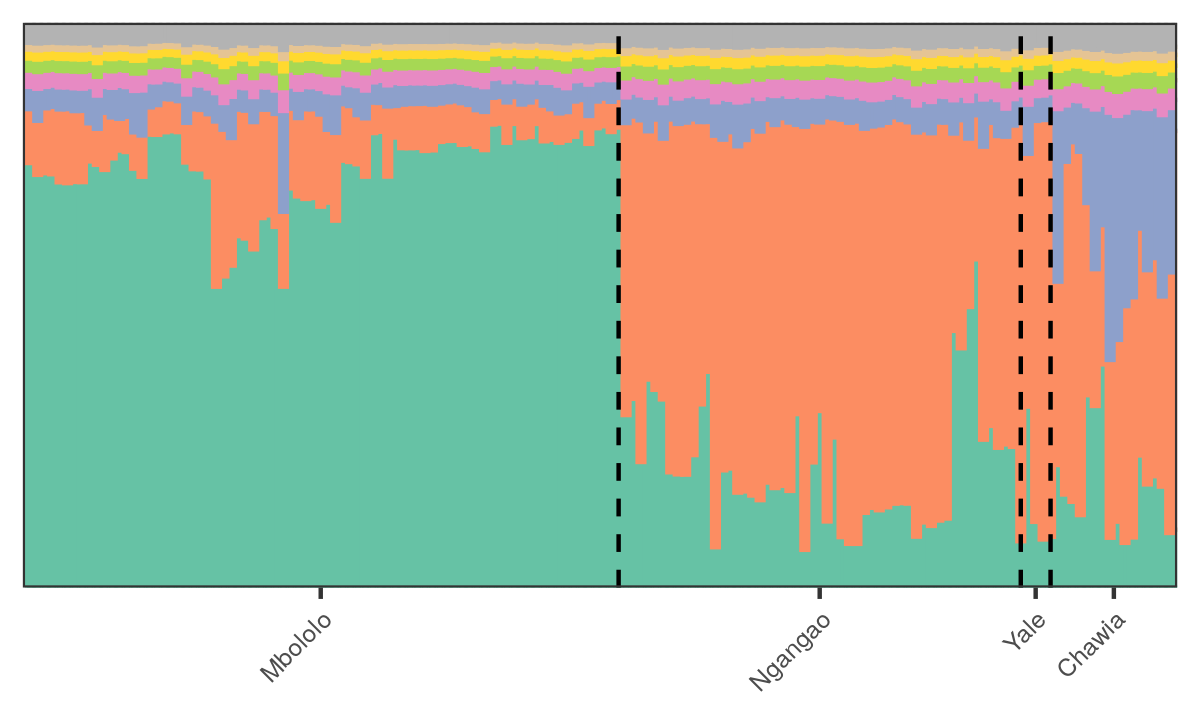
\includegraphics[width=0.980\linewidth,height=0.588\linewidth]{figure/stru_init_fit-1} 

}

\caption[The inferred individual admixtures at $\alpha_0 = 3$]{The inferred individual admixtures at $\alpha_0 = 3$. 
    Each vertical strip is an individual and each color
    a latent population.
    Lengths of colored segments represent the inferred admixture proportions.
    Individuals are ordered by the geographic region from which they were sampled
    (Mbololo, Ngangao, Yale, and Chawia).
    In the text, we refer to the green, orange, and purple latent populations 
    as population 1, 2, and 3, respectively. }\label{fig:stru_init_fit}
\end{figure}


\end{knitrout}


\subsubsection*{Sensitivity: expected number of populations}

We start by evaluating the sensitivity of the expected number of populations
to the $\alpha$ parameter in the $\betadist{\nu_{nk}\vert 1, \alpha}$ stick distribution. 
We focus on the in-sample quantity. 
Define the expected number of populations containing at least $\tau$ loci as
\begin{align*}
\gpop(\eta; t)
&= \expect{\q(\z\vert\eta)}{\sum_{k=1}^\kmax \ind{ 
\left(\sum_{n=1}^{\nindiv}
\sum_{l=1}^{\nloci}
\sum_{i=1}^2
\z_{\n l i \k}\right) > \tau}}.
\end{align*}
% 
% $\gpop$ counts a population as present if they contain at least $\tau$ loci. 
% When $\tau = 0$, $\gpop$ is equivalent to the expected in-sample number of clusters discussed in \secref{results_iris}, except the summation is now over individuals, loci, and chromosomes. 

At $\tau = 0$, $\gpop$ has a simple closed form expression as a function of the expectations of $\z_{\n l i \k}$; 
for $\tau > 0$, we resort to Monte Carlo estimates. 
Like the posterior quantity $\gclusterspred$ discussed in \secref{results_iris},
we use the re-parameterization trick to sample from $\q(\z\vert\eta)$. 
This allows us to condition on fixed draws from a distribution that is independent of $\eta$ (in this case the underlying distribution is $\mathrm{Uniform}[0, 1]$); 
these fixed draws are shared across every computation of $\gpop(\eta; t)$ below. 

The expected number of latent populations is sensitive to $\alpha$ (\figref{stru_alpha_nclusters}).
Without any thresholding ($\tau = 0$),
the expected number of populations quickly increases as $\alpha$ increases; 
in fact, it nearly saturates at $\kmax = 20$ when $\alpha = 7$. 
This sensitivity is likely due to the fact that the non-thresholded quantity 
is highly dependent on the behavior of small, nearly unoccupied populations;
even though the probability of a single locus belonging to these rare populations is small, the probability that \textit{none} of the $\nindiv \times \nloci \times 2$ observed genotypes belong to these rare populations is non-negligable.  

This motivates the use of thresholding in reporting the number of populations. 
We threshold at $\tau = 20$ and $\tau = 40$, corresponding to approximately 
$2\%$ and $4\%$ 
of the total number of loci in the data set, respectively. 
In the refits, the thresholded quantities still vary between two and four
latent populations. 

The linear approximation imperfectly captures the results observed by refitting. 
We formed the linear approximation at $\alpha_0 = 3$ and computed 
$\gpop$ at variational parameters $\etalin(\alpha)$ for $\alpha = 1, \ldots, 7$. 
For this range of $\alpha$, the linearly approximated and the refitted variational parameters almost perfectly agree on values of $\gpop$ with $\tau = 0$. 
However, substituting $\etalin(\alpha)$ for the refitted values $\etaopt(\alpha)$
underestimated the sensitivity of $\gpop$ when $\tau = 20$ and $\tau = 40$.  
In particular, the linearly approximated variatonal parameters failed to produce the reduction to two latent populations at $\alpha = 1$ observed in the refits.


\begin{knitrout}
\definecolor{shadecolor}{rgb}{0.969, 0.969, 0.969}\color{fgcolor}\begin{figure}[!h]

{\centering 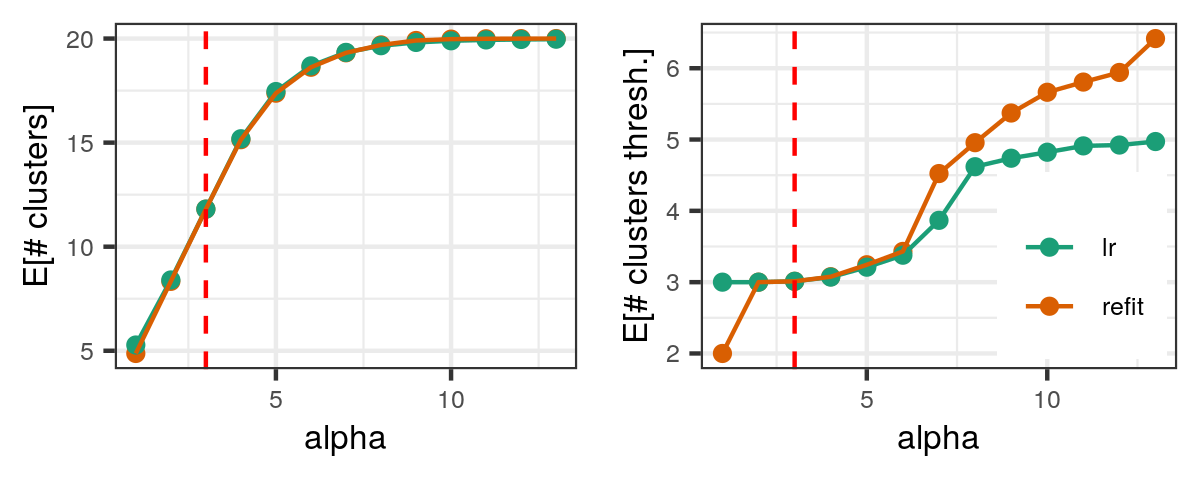
\includegraphics[width=0.980\linewidth,height=0.431\linewidth]{figure/stru_alpha_nclusters-1} 

}

\caption[The expected number of (thresholded) 
    populations in the thrush data as $\alpha$ varies.
    We computed the linear approximation at $\alpha_0 = 3$, and
    we compare the 
    results under the linearly approximated variational parameters with the
    results observed after refitting]{The expected number of (thresholded) 
    populations in the thrush data as $\alpha$ varies.
    We computed the linear approximation at $\alpha_0 = 3$, and
    we compare the 
    results under the linearly approximated variational parameters with the
    results observed after refitting. 
    Thresholds at $\tau = 20$ and $\tau = 40$ corresponding to 
    approximately 
    $2\%$ and $4\%$ 
    of the total number of loci in the data set, respectively. }\label{fig:stru_alpha_nclusters}
\end{figure}


\end{knitrout}

We provide some more intuition concerning the expected number of populations $\gpop$ with some threshold $\tau > 0$. 
$\gpop$ is closely related to the expected number of loci belonging to each population, defined as
\begin{align*}
\gloci(\eta; k)
&= \expect{\q(\z\vert\eta)}{\sum_{n=1}^{\nindiv}
\sum_{l=1}^{\nloci}
\sum_{i=1}^2
\z_{\n l i \k}}. 
\end{align*}

\figref{stru_alpha_cluster_weights} plots $\gloci$ for the first six populations 
as $\alpha$ varies.
The expected number of loci at the initial fit, $\gloci(\etaopt(\alpha_0); k)$,
is at least 100 for populations $\k = 1, 2,$ and $3$, 
while $\gloci(\etaopt(\alpha_0); k)$ is less than 
12
for the remaining populations.  
A sample of memberships $\z\sim \q(\z\vert\etaopt(\alpha_0))$ will 
almost always have at least $\tau$ loci allocated to populations 1, 2, and 3, 
while the allocations to each remaining population will almost always be below $\tau$, for either $\tau = 20$ or $\tau = 40$. 
Thus, at $\alpha = \alpha_0$ there then are clearly 3 populations as defined by our threshold.  

At $\alpha = 7$, the expected number of loci belonging to population 4
increases to 
$20.7$, 
a new population emerges above the threshold at $\tau = 20$. 
On the other hand, under the refitted variational parameters at $\alpha = 1$, 
the expected number of loci belonging to population 3 decreases to 
$6.7$, 
below the thresholds $\tau = 20$ and $\tau = 40$. 
Thus, the expected number of latent populations with
either threshold $\tau = 20$ or $\tau = 40$ decreases to two. 
The linear approximation under-estimated this decrease in allocation to
population 3, and 
therefore continued to predict three latent populations even at $\alpha = 1$. 


\begin{knitrout}
\definecolor{shadecolor}{rgb}{0.969, 0.969, 0.969}\color{fgcolor}\begin{figure}[!h]

{\centering 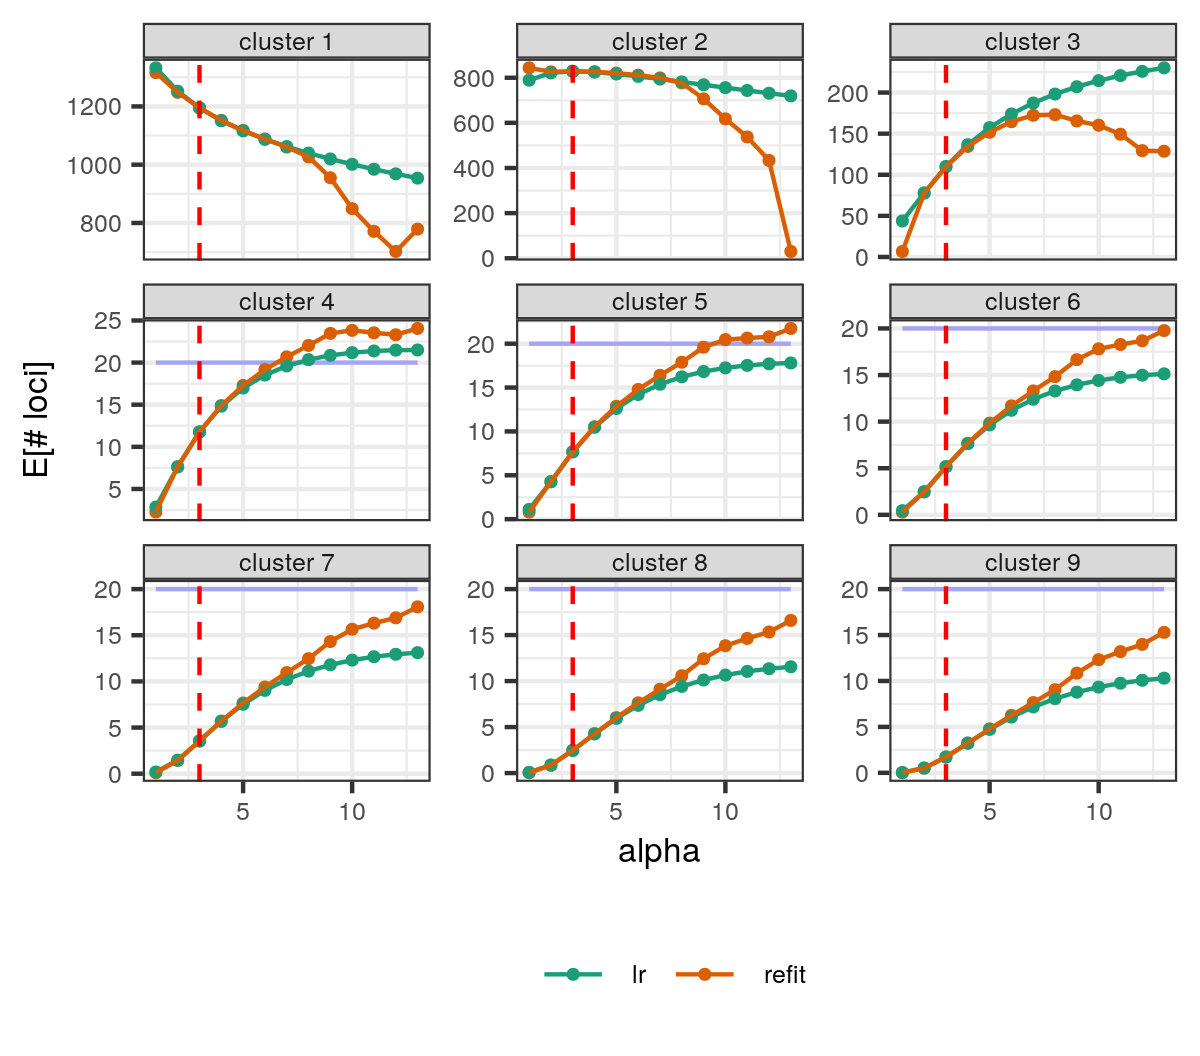
\includegraphics[width=0.980\linewidth,height=0.588\linewidth]{figure/stru_alpha_cluster_weights-1} 

}

\caption[The expected number of loci per population as $\alpha$ varies]{The expected number of loci per population as $\alpha$ varies. }\label{fig:stru_alpha_cluster_weights}
\end{figure}


\end{knitrout}

\subsubsection*{Sensitivity: individual admixtures}

Examining the inferred admixtures in \figref{stru_init_fit} provide clues into historical migration patterns of the genotyped individuals. 
For example, while individuals collected from the Mbololo region are inferred to primarily be admixed with population 1, 
there are a few individuals have abnormally large admixture proportions of population 2 than the rest. 
Conversely, while individuals collected from the Ngangao region are primarily population 2, several individuals have abnormally large admixture proportions of population 1. 
This suggests the presence of migration between the Ngangao and Mbololo regions. 

In this subsection, we evaluate the sensitivity of this conclusion to possible prior perturbations. 
We consider the posterior statistic 
\begin{align*}
\gadmix(\eta; \mathcal{N}, k) = 
 \expect{\q(\z\vert\eta)}{\frac{1}{|\mathcal{N}|}\sum_{n\in\mathcal{N}}
\pi_{\n\k}},
\end{align*}
the average admixture proportion of population $\k$ in a set of 
individuals $\mathcal{N}$. 

We present results on three variations of $\gadmix$: 
the six individuals from the Mbololo region with outlying proportions 
of population 2 ($\mathcal{N} = \{25, ..., 30\}, k = 2$); 
the four individuals from the Ngangao region with outlying proportions 
of population 1 ($\mathcal{N} = \{44, ..., 37\}, k = 1$); 
and all individuals from the Chawia region 
($\mathcal{N} = \{44, ..., 37\}, k = 3$). 
The first two cases are related to the question of migration between the Mbololo and Ngangao regions. 
In the last case, we are examining the sensitivity of the presense of the third population in the Chawia region. 

For each statistic, we construct the worst-case negative perturbation (negative because we are interested in making these patterns disappear). 
\figref{stru_func_sens} displays the effect of each worst-case perturbation on its respective posterior statistic. 
The linear approximation $\gadmix(\etalin(\epsilon); \mathcal{N}, k)$ 
predicts that the presence of population 2 in the outlying Mbololo individuals to be sensitive to this worst-case perturbation:
the admixture proportion of population 2 is nearly halved after the perturbation. 
The quantity computed by refitting the model confirms the prediction by the linear approximation. 
On the other hand, the presence of population 1 in the outlying Ngangao individuals appear to be insensitive, even after a worst-case perturbation. 
The linear approximation and the refits agree on this conclusion. 
Finally, the presence of population 3 in the Chawia individuals is anticipated to be sensitive under the linear approximation, as this admixture proportion steadily decreases as $\epsilon\rightarrow 1$ 
However, under the refits, this admixture proportion does not decrease steadily but rather levels off after $\epsilon = 0.5$. 



\begin{knitrout}
\definecolor{shadecolor}{rgb}{0.969, 0.969, 0.969}\color{fgcolor}\begin{figure}[!h]

{\centering 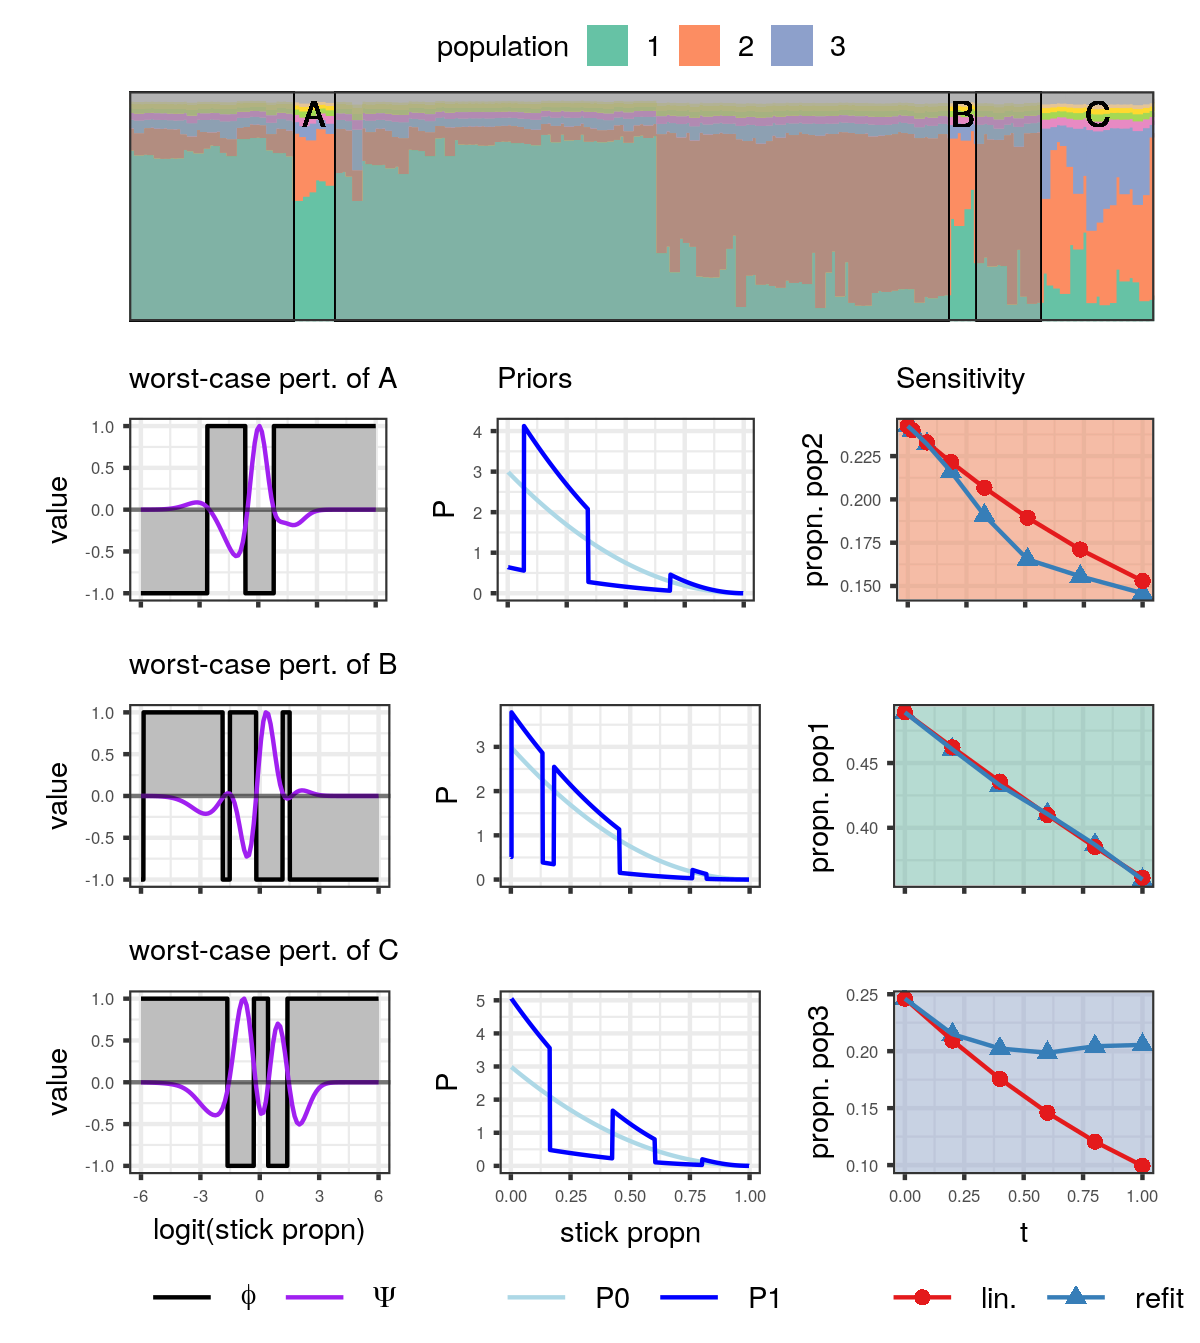
\includegraphics[width=0.980\linewidth,height=1.098\linewidth]{figure/stru_func_sens-1} 

}

\caption[Sensitivity of inferred admixtures for several outlying individuals]{Sensitivity of inferred admixtures for several outlying individuals. 
     For individuals A, 
     we examine the sensitivity of the admixture proportion of population 2.
     For individuals B, 
     we examine the population 1 admixture
     For the individuals C, we examine the population 3 admixture.
     (Left column) The worst-case negative perturbation with unit $L_\infty$-norm 
     in grey,
     plotted against the influence function in purple
     (scaled to also have $L_\infty$ norm equal to 1). 
    (Middle column) The effect of the perturbation on the prior density. 
    (Right column) Effects on the inferred admixture. }\label{fig:stru_func_sens}
\end{figure}


\end{knitrout}

discussion of overall findings

compute time. 

\begin{table}[tb]
\centering
\caption{Compute time of results on the structure dataset. }
\begin{tabular}{|r|r|}
\hline 
    & time (seconds) \\ 
    \hline 
    Initial fit & 7 \\
    \hline
    Hessian solve for $\alpha$ sensitivity & 
        0.32\\
    Linear approx. $\eta^{lin}(\alpha)$ for $\alpha = 1, ..., 10$ & 
        0.0059\\
    Refits $\eta(\alpha)$ for $\alpha = 1, ..., 10$ & 
        34\\
    \hline
    The influence function & 0.59\\
    Hessian solve for worst-case $\phi$ &
        0.38\\
    Linear approx. $\eta^{lin}(\epsilon)|_{\epsilon = 1}$ 
      for worst-case $\phi$ &
        0.00085\\
    Refit $\eta(\epsilon)|_{\epsilon = 1}$ 
      for worst-case $\phi$ &
        13\\
    \hline
\end{tabular}
\end{table}

\subsection{Limitations of local sensitivity}

In this final subsection, 
we discuss some examples where employing local sensitivity fails to reproduce
the changes in a posterior statistic observed by refitting. 
The linear approximation $\etalin(t)$, naturally, will be a poor subsitute when prior perturbation produces non-linear changes in $\etaopt(t)$. 
The examples discussed below use the STRUCTURE model and dataset presented in 
subsection above, and we consider the first perturbation shown in \figref{stru_func_sens}.

Recall from \figref{stru_func_sens} that the linear approximation agreed with the refit in predicting the admixture proportion of population 2 
in the outlying Mbololo individuals. 
We delve more closely into the inferred admixtures under both the refitted and linearly approximated variational parameters after this perturbation. 
While the linear approximation was able to capture the overall proportion of population 2 in the Mbololo individuals, 
the linear approximation does not perform uniformly well over all individuals 
(\figref{stru_func_sens_admix}). 
In particular, the admixture proportion of population 2 in individual $n = 25$ dramatically increased after this perturbation. 
The linear approximation failed to detect this change. 


\begin{knitrout}
\definecolor{shadecolor}{rgb}{0.969, 0.969, 0.969}\color{fgcolor}\begin{figure}[!h]

{\centering 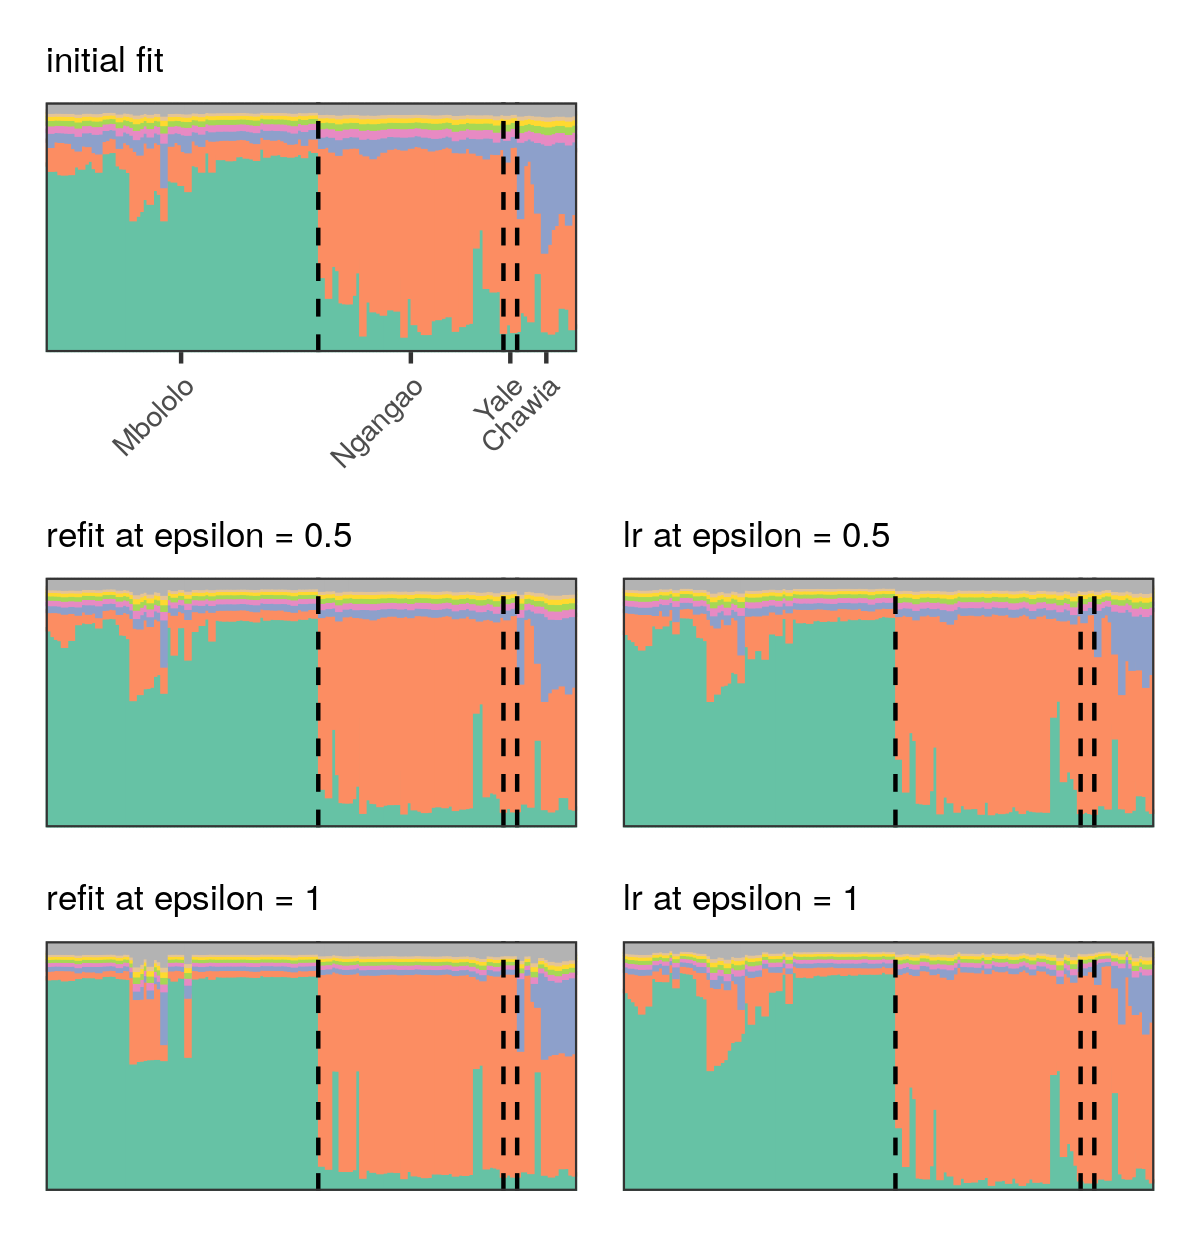
\includegraphics[width=0.980\linewidth,height=0.392\linewidth]{figure/stru_func_sens_admix-1} 

}

\caption{Inferred admixtures after the worst-case prior perturbation 
     to individuals A (second row, Figure~\ref{fig:stru_func_sens}). }\label{fig:stru_func_sens_admix}
\end{figure}


\end{knitrout}

\figref{stru_lin_bad_example_cap} examines this individual more closely. 
The bottom row plots this individual's admixture proportions as $\epsilon$ varies from 0 to 1. 
In the refit, the admixture proportion of population 1 decreased from 
0.53
to 
0.29, 
while the admixture proportion of population 2 increased from            
0.29
to 
0.56. 
The linearly approximated values failed to detect this change. 
The reason is because for this perturbation, the mapping from 
$\epsilon$ to the variational parameter on the stick-distribution governing the inferred admixtures is highly non-linear. 
The top row plots the location parameter of the logit-normal distribution 
as $\epsilon$ varies from 0 to 1. 
In our approximation, the location parameter is linear with respect to $\epsilon$. 
However, the true relationship between the location parameter of the first stick and $\epsilon$ as obtained by refitting is concave -- the location parameter increases at first, then decreases. 
Thus, the linear approximation expects the change in this location parameter to be positive when in fact it is negative. 
The corresponding admixture mixture proportion of population 1 is therefore mis-estimated by the linear approximation. 
Furthermore, the admixture proportion of population two depends on the first stick length. 
Because our linear approximation over-estimated the length of the first stick, 
and the second admixture proportion is a product of the second stick and remaining stick length after the first stick, 
the linear approximation then under-estimates the admixture proportion of population 2. 



\begin{knitrout}
\definecolor{shadecolor}{rgb}{0.969, 0.969, 0.969}\color{fgcolor}\begin{figure}[!h]

{\centering 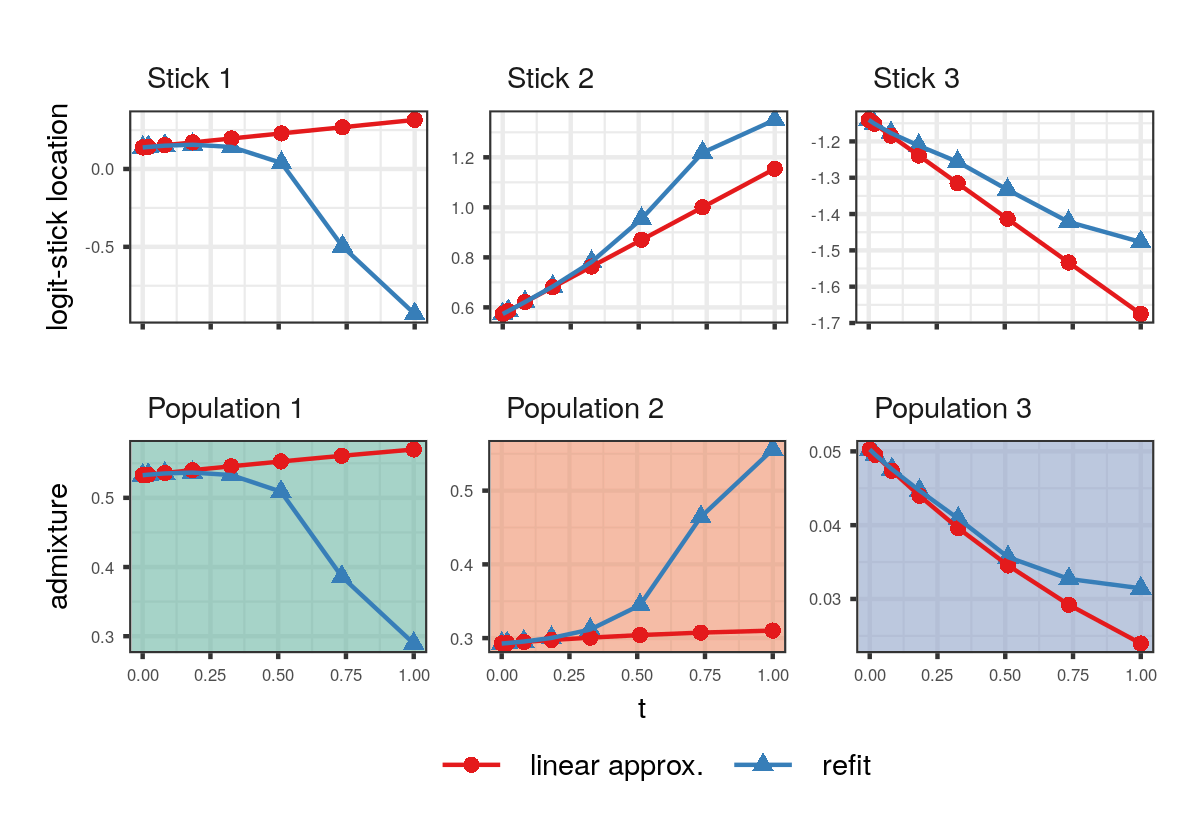
\includegraphics[width=0.980\linewidth,height=0.666\linewidth]{figure/stru_lin_bad_example-1} 

}

\caption[An example where the linear approimxation poorly captured the 
    change in the admixture proportions of individual $n = 25$]{An example where the linear approimxation poorly captured the 
    change in the admixture proportions of individual $n = 25$.}\label{fig:stru_lin_bad_example}
\end{figure}


\end{knitrout}



In the examples above, we only linearized the mapping $\epsilon \mapsto \etaopt(\epsilon)$. 
In most examples, we find that retaining the non-linearities from $\eta\mapsto g$ performed as well, or better than, fully linearizing the mapping from $\epsilon \mapsto \eta$. 
There are exceptions, as we discuss below. 


\begin{knitrout}
\definecolor{shadecolor}{rgb}{0.969, 0.969, 0.969}\color{fgcolor}\begin{figure}[!h]

{\centering 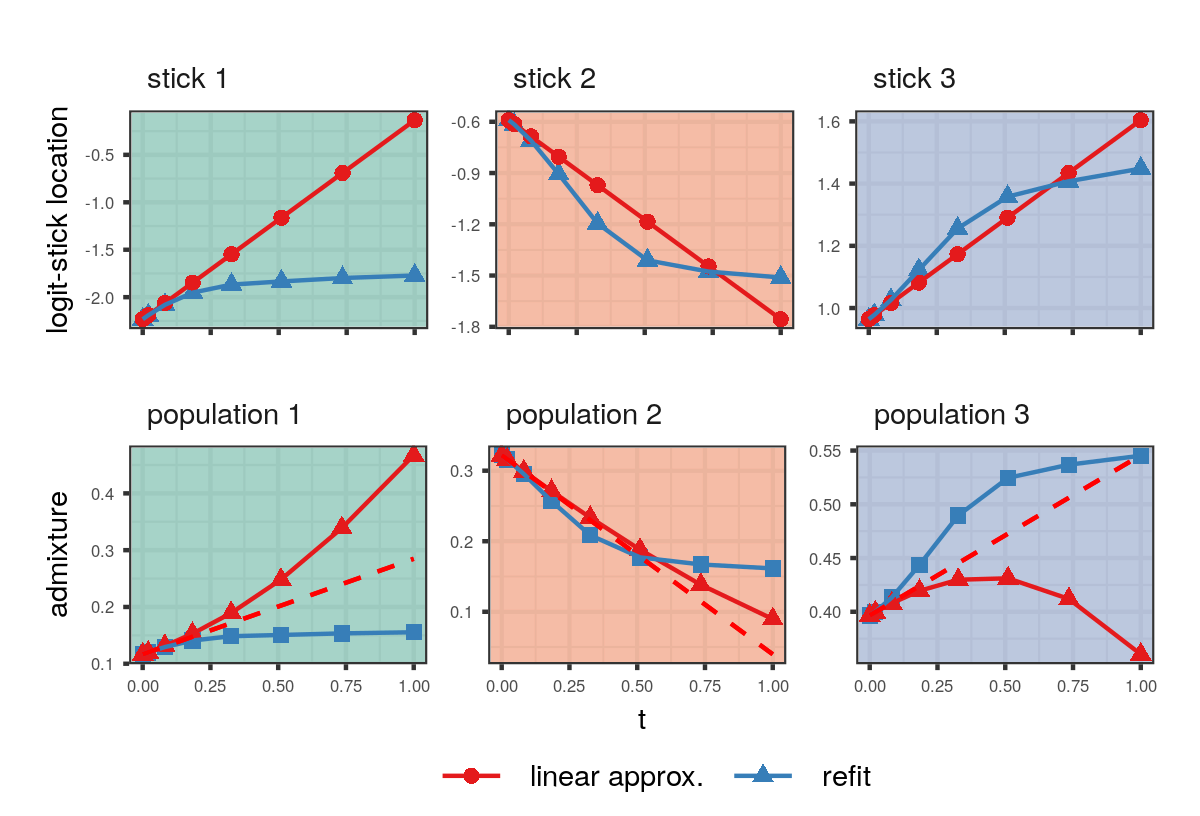
\includegraphics[width=0.980\linewidth,height=0.666\linewidth]{figure/stru_fully_lin_example-1} 

}

\caption[An example where a fully-linearizing the posterior statistic outperforms
    linearizing only the variational parameters]{An example where a fully-linearizing the posterior statistic outperforms
    linearizing only the variational parameters. 
    The fully-linearized approximation in dashed red produced an 
    accurate prediction of change in this individual's admxture proportion of
    population 3. }\label{fig:stru_fully_lin_example}
\end{figure}


\end{knitrout}





